\documentclass{beamer} 
\usepackage{amsmath,amsthm}
\usepackage{mathrsfs}
\usepackage{amssymb}
\usepackage[english]{babel}
\usepackage{latexsym}
\usepackage{amsfonts}
\usepackage{graphicx}
\usepackage{float}
\usepackage{graphics}
\usepackage{epsfig}
\usepackage{url}
\usepackage{soul}
\usepackage{listings}
\usepackage{bm}

% \usepackage{minted}


\usetheme{WVU}
\usecolortheme{WVU}
\usepackage{multirow}

\mode<presentation> 

\title[VE401 SU2022 RC week10]{VE401 SU2022 RC week10}

\author[ Shuyu Wu ]{ Shuyu Wu }
\institute[UM-SJTU JI]{UM-SJTU Joint Institute \vspace{.2cm} \\ 
\includegraphics[scale=0.3]{umji_logo.png}\\wushuyu2002@sjtu.edu.cn}
\date[July 2022]{\today}

\begin{document}
\begin{frame} 

\titlepage 

\end{frame} 
\section{Categorical Data}
\begin{frame}
    \frametitle{Outline}
    \tableofcontents[currentsection]
\end{frame}

\begin{frame}
    \frametitle{Categorical Random Variables}
    It's the generalization of 0-1 (or Bernolial) distribution, in terms of Categories(not only success or failure).\par
    That means $X$ can take value $1,2,\dots , k$, each with probability $p_1, p_2, \dots , p_k$, and we have $\sum\limits_{i=1}^{k}p_i=1$, of course.\par
    A random sample of size n from $X$ is collected and the results are
    expressed as a random vector $(X_1, X_2, \dots , X_k)$, and $X_i$ means the count that $X=i$. 
    

\end{frame}

\begin{frame}
    \frametitle{Multinomial Trials}

    A multinomial trial with parameters $p_1,\dots ,  p_k$ is a trial
    that can result in exactly one of k possible outcomes. The probability that
    outcome i will occur on a given trial is $p_i$, for $i=1,\dots , k$.\par
    A multinomial random variable now counts the number of times that
    outcome i occurs when a fixed number of n i.i.d. multinomial trials is performed.

\end{frame}

\begin{frame}
    \frametitle{The Multinomial Distribution}

    A random vector $(X_1, X_2, \dots , X_k)$ with joint PDF 
    \[f_{X_1, X_2, \dots , X_k}(x_1, x_2, \dots , x_k)=\frac{n!}{x_1! x_2!\dots x_k!}p_1^{x_1}\dots p_k^{x_k}\]

\end{frame}

\begin{frame}
    \frametitle{Chi-squared Goodness-of-fit Test}

    \textbf{Pearson statistic}: In a multinomial distribution, when n is large, $\sum\limits_{i=1}^{k}\frac{(X_i-np_i)^2}{np_i}\sim \chi^2_{k-1}$ approximately.\par
    \vspace{0.3cm}
    Then, for a null hypothesis ``$(X_1, X_2, \dots , X_k)$ follows a multivariate distribution with parameters $p_1, p_2, \dots , p_k$", we can apply such chi-squared test to test it.\par
    We may notice that $np_i$ is the ``expected value'', $X_i$ is the obeserved value. Denote them as $E_i$ and $O_i$, the pearson statistic is 
    \[\sum\limits_{i=1}^{k}\frac{(O_i-E_i)^2}{E_i}\]

\end{frame}

\begin{frame}
    \frametitle{Chi-squared Goodness-of-fit Test}
    For null hypothesis $H_0: p_i=p_{i0}$ in multinomial distribution, the test statistic is
    \[\chi^2_{k-1}=\sum\limits_{i=1}^{k}\frac{(X_i-np_{i0})^2}{np_{i0}}\]
    And we treat it as a one-tail test, so we reject $H_0$ at significance level $\alpha$ if $\chi^2_{k-1}>\chi^2_{\alpha, k-1}$. Or you can calculate a p-value.

\end{frame}

\begin{frame}
    \frametitle{ex 10.1}

    $X$ is believed to follow a multinomial distribution with parameters 0.1, 0.2, 0.3, 0.4. performe 100 multinomial trials and the outcome is 13 ``1'', 22 ``2'', 25 ``3'' and 40 ``4''. What's your conclusion?

\end{frame}

\begin{frame}
    \frametitle{ex 10.1 answer}

    We have $E_1=10, E_2=20, E_3=30, E_4=40$, and $O_1=13, O_2=22, O_3=25, O_4=40$. So the Pearson chi-squared statistic is 
    \[\frac{(13-10)^2}{10}+\frac{(22-20)^2}{20}+\frac{(25-30)^2}{30}+0=1.93\]
    The degree of freedom is 4-1=3. The p-value is 0.587, so there's of course no evidence that the data doesn't follow such distribution.

\end{frame}

\begin{frame}
    \frametitle{Goodness-of-Fit Test for a Discrete Distribution}

    Such method can also be generalized to any discrete distribution, for example, geometric or Poisson distribution, bacause thay can be regarded as a multinomial distribution with $k=\infty$. We calculate the expected value $E_i$ and get observed value $O_i$ for $i$ that satisfy Cochran's Rule.\par
    \vspace{0.3cm}
    \[\sum\limits_{i=1}^{k}\frac{(O_i-E_i)^2}{E_i}\]
    will follow a chi-squared distribution with $k-1-m$ degrees of freedom. m is the parameters that we estimated.\par
    Please notice that $O_i$ must be directly observed, it shouldn't be processed. For example, you shouldn't use the proportion instead of the real value. In ex 10.1, you shouldn't test 0.13, 0.22, 0.25, 0.4 against 0.1, 0.2, 0.3, 0.4. That won't work at all!
    

\end{frame}

\begin{frame}
    \frametitle{Goodness-of-Fit Test for a Continuous Distribution}
    Bin the range to turn it into discrete random variable. You'd better use software, otherwise it may take a long time.
    

\end{frame}

\begin{frame}
    \frametitle{Test of Independence}

    If two groups of data are independent, their joint distribution is the product of marginal density. So, we can calculate out the marginal density by summing one row/column up and divide by total sample size.\par
    Suppose two categories are independent, then the joint density should be their product, and we can calculate the ``expected value''. Finally we can perform the chi-squared test. The degree of freedom is $(r-1)(c-1)$.

\end{frame}

\begin{frame}
    \frametitle{ex 10.2}

    Within 100 people, set X to be their gender and Y to be their dominant hand. We get the following result:

\begin{table}[H]
    \centering
      \begin{tabular}{lrrr}
            & \multicolumn{1}{l}{male} & \multicolumn{1}{l}{female} & \multicolumn{1}{l}{total} \\
      right-handed & 43    & 44    & 87 \\
      left-handed & 9     & 4     & 13 \\
      total & 52    & 48    & 100 \\
      \end{tabular}%
    
  \end{table}%
  Is there evidence that X and Y are not independent?
\end{frame}

\begin{frame}
    \frametitle{ex 10.2 answer}

    We calculate the expected value if they're independent:
    \begin{table}[H]
        \centering
          \begin{tabular}{lrrr}
                & \multicolumn{1}{l}{male} & \multicolumn{1}{l}{female} & \multicolumn{1}{l}{total} \\
          right-handed & 0.52*0.87*100=45.24    & 41.76    & 0.87 \\
          left-handed & 6.76     & 6.24     & 0.13 \\
          total & 0.52    & 0.48    & 1 \\
          \end{tabular}%
        
      \end{table}
      The degree of freedom is $(2-1)(2-1)=1$, and the test statistic is $\frac{(43-45.24)^2}{45.24}+\frac{(44-41.76)^2}{41.76}+\frac{(9-6.76)^2}{6.76}+\frac{(4-6.24)^2}{6.24}=1.777$, and we get the p-value 0.1825. So there's no evidence that $X$ and $Y$ are not independent.

\end{frame}

\section{Simple Linear Regression I:
Basic Model and Inferences}
\begin{frame}
    \frametitle{Outline}
    \tableofcontents[currentsection]
\end{frame}

\begin{frame}
    \frametitle{Linear Regression}

    Encouraged tool: matlab (with curve fitting toolbox)\par
    \vspace{0.3cm}
    We have a dependent random variable $Y$ and an independent random variable $X$. $Y$ is related to the value of $X(=x)$, denoted as $Y|x$.\par
    A linear model means we claim that
    \[\mu_{Y|x}=\beta_0+\beta_1 x\]
    or $Y|x = \beta_0+\beta_1 x +E$ and $E[E]=0$. $E$ is called noise and supposed to follow a normal distribution.\par
    We want to find estimators for $\beta_0$ and $\beta_1$, denoted as $B_0$ and $B_1$. Their estimates are denoted as $b_0$ and $b_1$. \par
    Question: what's their difference? Which of them are random variables? Why do we introduce so many variables?

\end{frame}

\begin{frame}
    \frametitle{Residuals}

    We get n pairs of data $(x_i, Y_i)$ $(i=1,2,\dots , n; Y_i:=Y|x_i)$. And we have 
    \[Y_i=b_0+b_1 x_i+e_i\]
    And our choice of $b_0$ and $b_1$ should minimize $e_i$.

\end{frame}

\begin{frame}
    \frametitle{Least-Squares Estimation}

    For $e_1, e_2, \dots , e_n$, we need to select proper $b_0$ and $b_1$ such that 
    \[SS_{E}=\sum\limits_{i=1}^{n} e_i^2=\sum\limits_{i=1}^{n} (y_i-(b_0+b_1 x))^2\]
    is minimized.\par
    The result is shown below:

\end{frame}

\begin{frame}
    \frametitle{Least-Squares Estimation Result}

    Set 
    \[\overline{x}=\frac{1}{n} \sum\limits_{i=1}^{n} x_i, \overline{y}=\frac{1}{n} \sum\limits_{i=1}^{n} y_i\]
    \[S_{xx}=\sum\limits_{i=1}^{n}(x_i-\overline{x})^2, S_{yy}=\sum\limits_{i=1}^{n}(y_i-\overline{y})^2, S_{xy}=\sum\limits_{i=1}^{n}(x_i-\overline{x})(y_i-\overline{y})\]
    And we have 
    \[b_1=\frac{S_{xy}}{S_{xx}}, b_0=\overline{y}-b_1 \overline{x}, SS_E=S_{yy}-b_1 S_{xy}\]

\end{frame}

\begin{frame}
    \frametitle{ex 10.3}

    x=[1  2  3  4  5  6  7  8  9 10 11 12 13 14 15 16 17 18 19 20]\par
    y=[1.01332169  2.58854276  5.2414765   5.7702422   6.65249669  7.87463635
    9.31371493 10.35293335 11.21191426 12.85894351 13.74200276 15.87336542
   16.59916645 18.03548874 19.42891692 20.17796239 21.22333748 23.65158877
   23.25779558 26.15827289]\par
   Perform a linear regression.

\end{frame}

\begin{frame}
    \frametitle{ex 10.3 answer}

    Method 1: use curve fitting toolbox.\par
    \begin{figure}[H]
        \centering
        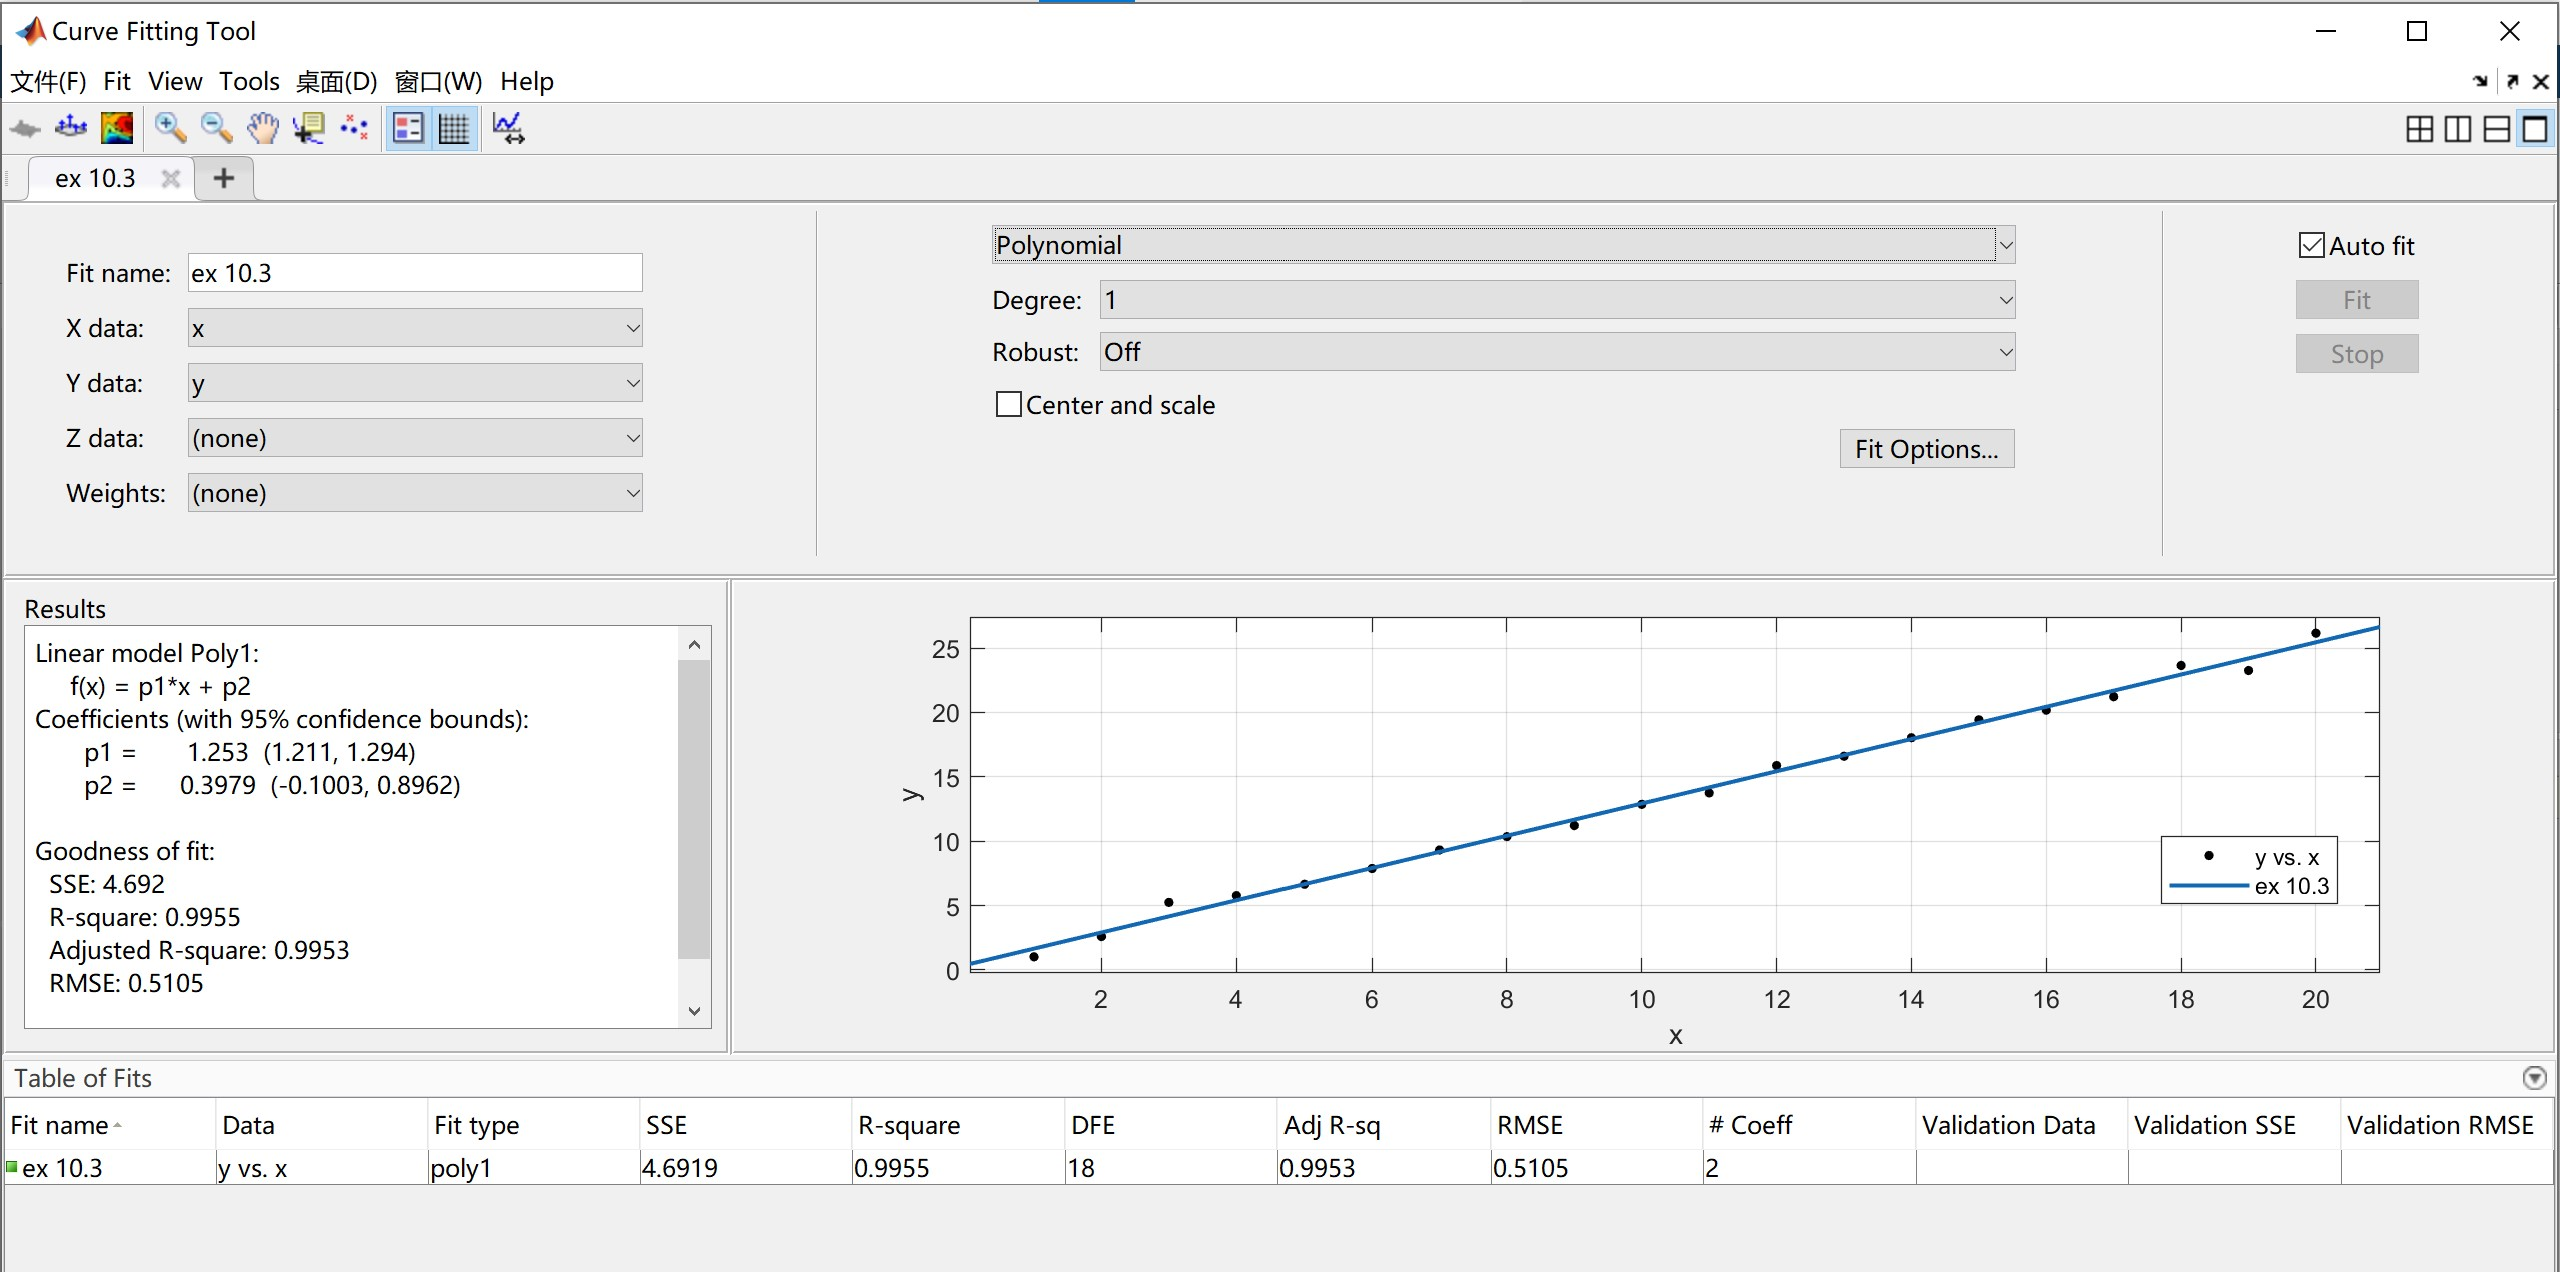
\includegraphics[width=0.6\textwidth,height=0.3\textwidth]{ex10_3_m1.jpg}
        \caption{fitting result}
    \end{figure}\par
    So we have $b_0=0.3979, b_1=1.253$, $SS_E=4.692$

\end{frame}

\begin{frame}
    \frametitle{ex 10.3 answer}

    Method 2: direct calculation\par
    $\overline{x}=10.5$, $\overline{y}=13.55$. $S_{xx}=665$, $S_{yy}=1048.3$, $S_{xy}=833.05$\par
    So $b_1=1.2527$, $b_0=0.3979$, $SS_E=4.6919$.

\end{frame}

\begin{frame}
    \frametitle{Estimate Residuals}

    Now we focus on the residual generated by $E$. $E\sim N(0,\sigma^2)$. The sample variance of $E$ is 
    \[S^2=\frac{SS_E}{n-2}\]
    which is an unbiased estimator of $\sigma^2$. \par
    

\end{frame}

\begin{frame}
    \frametitle{Tests for Regression Parameters}
    The confidence interval for $\beta_0$ and $\beta_1$ are:
    \[\beta_1: b_1\pm t_{\alpha/2, n-2} \frac{S}{\sqrt{S_{xx}}}\]
    \[\beta_0: b_0\pm t_{\alpha/2, n-2} \frac{S \sqrt{\sum x_i^2}}{\sqrt{n S_{xx}}}\]
    We say that a regression is significant if there is statistical evidence that
    the slope $\beta_1\neq 0$, that is to say, the confidence interval of $\beta_1$ doesn't contain 0.
    

\end{frame}

\section{Extra topic and Q\&A}
\begin{frame}
    \frametitle{Outline}
    \tableofcontents[currentsection]
\end{frame}



\begin{frame}
    \frametitle{Q\&A}
    
    Feel free to ask if you have any questions.\par
    
    
    
\end{frame}

\end{document} 